\section{Assurance on Data}\label{sec:datapreparation}

Most efforts on the analysis of machine learning models, as we discussed in previous chapters, are on the trained models. This is based on an assumption that, the trained models have taken into consideration all necessary information from the training dataset; no more, no less. Any deviation from this assumption may lead to the analysis results not applicable to the machine learning development cycle. For example, if the generated test cases are not on the same distribution with the training data, then the reliability assessment results (Section~\ref{sec:safetyassurance}) such as the failure rate based on the test cases will not be valid. If the training dataset does not conform with the operational data distribution, then the empirical generalisation error will not be a good approximation to the true generalisation error (Section~\ref{sec:generalisationerror}). There are also some safety vulnerabilities such as data poisoning that cannot be detected simply from a trained model. While an exact computation, or even an  estimation, on the deviation is hard to achieve, we believe a few  data processing steps are useful as \emph{good practice} to improve the quality of training data and are therefore essential for safety assurance of machine learning. These steps include data cleaning, data pre-processing, data augmentation, and data anomaly detection. Figure~\ref{fig:dataquality} provides an illustrative diagram showing the flow of data in these steps. 

\begin{figure}[!htbp]
    \centering
    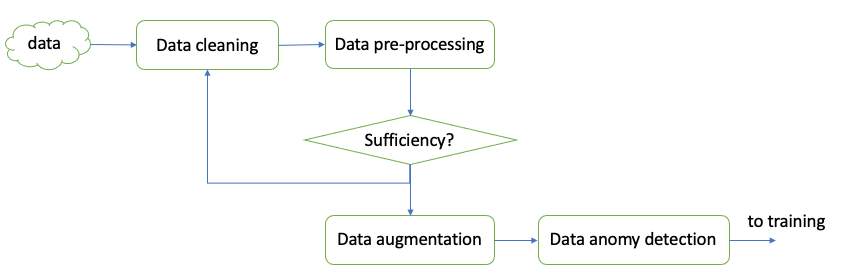
\includegraphics[width=\textwidth]{images/LookFurther/dataquality.png}
    \caption{Assurance on Data}
    \label{fig:dataquality}
\end{figure}

%
\emph{Data cleaning} is a process of ensuring that data is correct, consistent and usable. There are some recent good practices in industry. For example, \cite{10.14778/3229863.3229867} discusses a good practice in Amazon on automating the data validation process, where the quality of data is measured from three aspects: completeness, consistency, and accuracy. The completeness refers to the degree to which a data instance includes data required to describe a real world object, the consistency is defined as the degree to which a set of semantics rules are violated, and the accuracy is the correctness of the data. A set of pre-defined constraints are utilised by the user to define more involved data quality constraints, over which one can determine the quality of a dataset. 

After passing the data cleaning, the dataset is \emph{pre-processed} with  a few typical methods, such as standarisation, normalisation,  whitening, and decorrelation. These techniques are to optimise the dataset in order to help machine learning algorithms to achieve better performance. 
%

The data cleaning and pre-processing steps will result in a dataset that can be utilised for training. However, we still need to ensure that, for a  target machine learning algorithm, the data is sufficient for training a good model. Different machine learning algorithms may have different data sufficiency requirements. A principled decision process (to be discussed further in Section~\ref{sec:trainingsufficiency}) is required to determine the sufficiency of training data. If it is believed that the training data is insufficient, additional efforts may be needed on data collection. On the other hand, for some safety properties such as the robustness, additional data may come from  \emph{data augmentation}, which generates more data during the training phase so that the resulting trained model performs better on the safety property. However, unlike safety properties, extra care is needed to use data augmentation for the improvement of the accuracy of the model, because it will risk losing the i.i.d. property of training data. 

Finally, related to the safety of machine learning, we need to be mindful on the potential of data poisoning and backdoor attacks, and it is recommended that some techniques (as we discussed in the previous chapters) for the detection and reduction of such risks would be desirable.  Along this line, \cite{DBLP:conf/mlsys/BreckP0WZ19} considers a good practice at Google on the quality of data that will be fed into machine learning pipeline. It mainly focuses on utilising an anomaly detector to deal with challenges such as unexpected patterns, schema-free data, and training/serving skew. 

\subsection*{Expected Outcome}

The resulting dataset is required to be complete, consistent, accurate, optimised, sufficient, and free from outliers and poisoning data. All these properties can, and should, be objectively evaluated. We remark that, there are other requirements, such as balanced data and data diversity, which are also desirable to have 
%but can be arguable to be necessary 
for the safety assurance. If additional requirements are to be imposed, objective measurements and validation methods are needed. 